\section{Lec 17}
\subsection{Geodesic of Schwarzschild}
We derived the metric 
\[
ds^{2} = - \left( 1- \frac{2GM}{r} \right)dt^{2} + \left( 1- \frac{2GM}{r} \right)^{-1}dr^{2} + r^{2} d\Omega ^{2}
\]
now, the geodesic for test particles is
\[
\frac{d^{2} x^{\mu }}{d \lambda ^{2}} + \Gamma ^{\mu }_{\alpha \beta } \frac{d x^{\alpha }}{d \lambda }\frac{d x^{\beta }}{d \lambda } = 0
\]
In the Newtonian limit there are two quantities that are the \emph{effective potential}, that combines multiple effect into a single potential. It is defined as
\[
V_{eff}\left( r \right) = \frac{L^{2}}{2mr^{2}} - \frac{GMm}{r}
\]
where \emph{L} is the angular momentum, \emph{r} is the distance between the two masses, \emph{m} is the mass of the orbiting body and the second term is the potential.
There is the \emph{energy, E}
\[
	E = \frac{1}{2}m\dot{r}^{2} + V_{eff}\left( r \right)
\]
we said about geodesic that they're a trajectory that parallel transport  the momentum vector
\[
p^{\nu }\nabla _{\nu }p^{\mu } = 0
\]
lower one index, so
\[
p^{\nu }\nabla _{\nu }g^{\mu \alpha } p_{\alpha  } = 0
\]
this is null also because of metric compatibility. I think this means that I can bring in the metric without spoiling the result. We remember that $p^{\nu } \equiv \frac{d x^{\nu }}{d \lambda }$.
The equation will go in this way
\begin{align}
	p^{\nu }\nabla _{\nu }p_{\mu } &= 0 \nonumber \\
	p^{\nu }\left[ \partial_{\nu }p_{\mu } - \Gamma ^{\sigma }_{\nu \mu }p_{\sigma } \right] & = 0 \nonumber \\
	\frac{d x^{\nu }}{d \lambda } \partial_{\nu }p_{\mu } &= \Gamma ^{\sigma }_{\nu \mu }p^{\nu }p_{\sigma } \nonumber \\
	\frac{d x^{\nu }}{d \lambda }\frac{d }{d x^{ \nu }}p_{\mu } & = \Gamma ^{\sigma }_{\nu \mu }p^{\nu }p_{\sigma } \nonumber\\
	\frac{d p_{\mu }}{d \lambda } &= \Gamma ^{\sigma }_{\nu \mu } p_{\sigma }p^{\nu } \nonumber\\
	\frac{d p_{\mu }}{d \lambda } &= \frac{1}{2}g^{\sigma \rho } \left[ \partial_{\nu }g_{\rho \mu } + \partial_{\mu }g_{\rho \nu } - \partial_{\rho }g_{\mu \nu } \right] p_{\sigma }p^{\nu } \nonumber \\
				      &= \frac{1}{2} p^{\nu }p^{\rho } \left[ \partial_{\mu }g_{\rho \nu } \right] \nonumber \\
				     \frac{d p_{\mu }}{d \lambda } &= \frac{1}{2} \partial_{\mu }\left( g_{\rho \nu } \right) p^{\rho }p^{\nu } \\
\end{align}
What does it mean? Imagine there is a coordinate that does not appear in $g_{\mu \nu }$.
In fact looking at the expression of the metric at the start of the lecture, the metric does not explicitly depend on \emph{t}. This corresponds to the stationarity of the Schwarzschild spacetime. The conserved quantity associated with this symmetry is the particle's energy \emph{E} related to \emph{p\textsubscript{t}}.\par
Same for the azimuthal angle $\phi $, the metric does not explicitly depend on it. It correspond to the spherical symmetry of this spacetime, invariance under rotation around the central mass. The conserved quantity associated with this symmetry is $p_{\phi }$.\par
Still because of spherical symmetry we can focus on trajectories such that $\theta  = \frac{\pi }{2}$, without loss of generality.

\subsubsection{Gravitational Redshift}
We put ourselves on Earth, far away from $R_{S}$.
\begin{center}
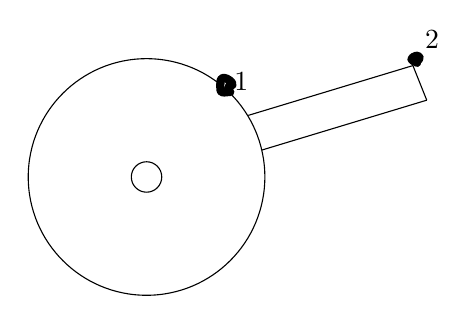
\begin{tikzpicture}[x=0.5pt,y=0.5pt,yscale=-1,xscale=1]
\draw   (240,154.5) .. controls (240,107.28) and (278.28,69) .. (325.5,69) .. controls (372.72,69) and (411,107.28) .. (411,154.5) .. controls (411,201.72) and (372.72,240) .. (325.5,240) .. controls (278.28,240) and (240,201.72) .. (240,154.5) -- cycle ;
\draw   (314.5,154.5) .. controls (314.5,148.42) and (319.42,143.5) .. (325.5,143.5) .. controls (331.58,143.5) and (336.5,148.42) .. (336.5,154.5) .. controls (336.5,160.58) and (331.58,165.5) .. (325.5,165.5) .. controls (319.42,165.5) and (314.5,160.58) .. (314.5,154.5) -- cycle ;
\draw    (409,135) -- (528,99) ;
\draw    (399,110) -- (518,74) ;
\draw    (518,74) -- (528,99) ;
\draw  [line width=3] [line join = round][line cap = round] (386,93) .. controls (383.64,93) and (379.29,94.34) .. (379,92) .. controls (378.71,89.68) and (378.71,87.32) .. (379,85) .. controls (379.8,78.56) and (393.19,89) .. (385,89) ;
\draw  [line width=3] [line join = round][line cap = round] (521,72) .. controls (521,71.41) and (514.41,70.15) .. (518,68) .. controls (524.18,64.29) and (523.85,71) .. (520,71) ;
\draw (387,77) node [anchor=north west][inner sep=0.75pt]   [align=left] {1};
\draw (525,47) node [anchor=north west][inner sep=0.75pt]   [align=left] {2};
\end{tikzpicture}
\end{center}
\bigskip
We emit a photon from the bottom to the top of the tower, of frequency $\nu $, we will find the relation between $\omega _{1}, \omega _{2}$.\par
This is a radial trajectory, this means that $d\phi =0$.
Now we will unravel the conserved quantity $p_{t}$
\begin{gather*}
	p_{t} = g_{t\alpha }p^{\alpha } = g_{tt} p^{t} \\
	p_{t} = - \left( 1- \frac{2GM}{r} \right) \frac{d t}{d \lambda } = \text{ const } = \alpha  
\end{gather*}
Now the goal is to find what $\omega _{1}$ is. I am sitting on 1. I want to achieve the first frequency $\omega _{1}$. In LIC we have
\begin{gather*}
u^{\hat{\mu }} = \left( 1,0,0,0 \right) \\
p^{\hat{\mu }} = \left( \omega , \omega \hat{n} \right)
\end{gather*}

The angular frequency is given by 
\[
\omega  = - u^{\hat{\mu }}p_{\hat{\mu }}
\]
but this has to be true in every coordinate system so
\[
\omega  = -u^{\mu }p_{\mu }
\]
Now, what we want is to know what is the angular frequency observed by observer.
He has four velocity 
\[
u^{\mu } = \left( 1,0,0,0 \right)
\]
and we know that 
\[
u^{\mu }u_{\mu } = -1
\]
since almost all the components are null we get the same writing
\[
g_{00}u^{0}u^{0} = -1
\]
and this leads us to find
\[
\omega = - g_{00}u^{0}p^{0} = \left( 1- \frac{2GM}{r} \right)\left( 1- \frac{2GM}{r} \right)^{-\frac{1}{2}} \frac{d t}{d \lambda } = \alpha \left( 1 - \frac{2GM}{r} \right)^{-\frac{1}{2}}
\]
so, as the photon moves radially, its energy will change.
\begin{equation}
\frac{\omega _{2}}{\omega _{1}} = \frac{\left( 1 - \frac{2GM}{r_{1}} \right)^{\frac{1}{2}}}{\left( 1- \frac{2GM}{r_{2}} \right)^{\frac{1}{2}}} \approx 1 - \frac{GM}{r_{1}} + \frac{GM}{r_{2}} = 1 - \Delta \phi 
\end{equation}
or 
\[
\frac{\Delta \omega }{\omega } = - \Delta \phi 
\]
where this $\phi $ is the gravitational potential, not a coordinate.

\subsubsection{Planets}

Most of the experimental tests of GR involve the motion of test particles in the solar system, Einstein suggested three tests two of which are the gravitational redshift, we talked about it above and the precession of perihelia. Now we will study the latter. To start we need to understand how the motion in the plane of the ecliptic works and in particular how to describe orbits in this particular metric, the Schwarzschild one.\par
Since the orbits are elliptical we need to express the radius \emph{r} in terms of the azimuthal angle $\phi $. \par
We shall start from two conserved quantities along the geodesics we mentioned before, $p_{t} = - E, p_{\phi } = L$.
\[
p_{t } = g_{tt}p^{t} = - \left( 1- \frac{2GM}{r} \right) \frac{d t}{d \lambda } = - E
\]
and 
\[
p_{\phi } = g_{\phi \phi } p^{\phi } = r^{2} sin^{2}\theta \frac{d \phi }{d \lambda } = r^{2} \frac{d \phi }{d \lambda } = L
\]
both quantities are expressed \emph{per unit mass}.\par
We know that the four velocity satisfies the normalization condition
\[
g_{\mu \nu }u^{\mu }u^{\nu } = - \epsilon_{r}
\]
where $\epsilon_{r}$ is a place-holder that
\[
\epsilon _{r} = \begin{cases}
 0 \text{ if massless particle }\\
 +1 \text{ if massive particle}
\end{cases}
\]
Now we apply the normalization in the Schwarzschild metric so
\begin{equation}
g_{tt}\left( \frac{d t}{d \lambda } \right)^{2} + g_{rr}\left( \frac{d r}{d \lambda } \right)^{2} + g_{\phi \phi }\left( \frac{d \phi }{d \lambda } \right)^{2}  = - \epsilon_{r}
\end{equation}
by substituting the conserved quantities and their friends we got
\begin{equation}
-\left( 1- \frac{2GM}{r} \right) \frac{E^{2}}{\left( 1- \frac{2GM}{r} \right)^{2}} + \frac{1}{\left( 1 - \frac{2GM}{r} \right)}\left( \frac{d r}{d \lambda }\right)^{2} + \frac{r^{2}L^{2}}{r^{4}} = - \epsilon_{r}
\end{equation}
with some manipulation,
\begin{equation}
\frac{1}{2}E^{2} = \frac{1}{2} \left( \frac{d r}{d \lambda } \right)^{2} + \left( 1- \frac{2GM}{r} \right)\left( \frac{\epsilon }{2} + \frac{L^{2}}{2r^{2}} \right)
\end{equation}
the second term of the right-hand side is $V_{eff}\left( r \right)$, the effective potential that holds effects of gravity and angular momentum, while the first term on the right is the radial kinetic energy.
\begin{equation}
\frac{1}{2} \left( \frac{d r}{d \lambda } \right)^{2} + V_{eff}\left( r \right) = \frac{1}{2}E^{2} = \mathcal{E} 
\end{equation}
Let's focus on this potential
\begin{equation}\label{eq:566}
V_{eff}\left( r \right) = \frac{\epsilon }{2} + \frac{L^{2}}{2r^{2}}- \frac{\epsilon GM}{r} - \frac{GML^{2}}{r^{3}}
\end{equation}
the first term is constant, the second is centrifugal, the third is newtonian and the fourth is GR's son.\par

\bigskip
\begin{minipage}{0.47\textwidth}
	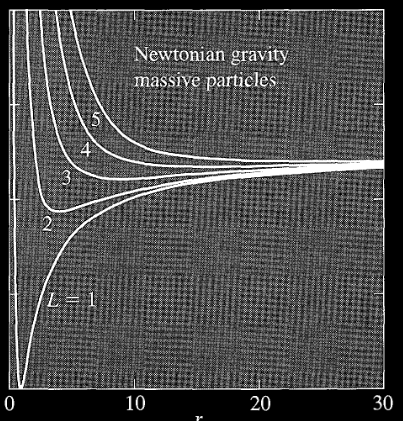
\includegraphics[width=0.8\linewidth]{imm/newtmassive.png}
	\label{fig:sub1}
\end{minipage}
\hfill
\begin{minipage}{0.47\textwidth}\label{fig:vrvsr}
	 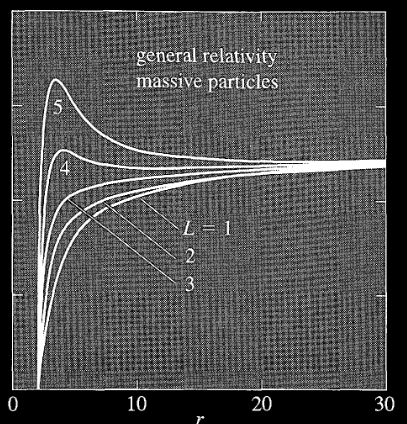
\includegraphics[width=0.8\linewidth]{imm/grmassive.png} 
	\label{fig:sub2}
 \end{minipage}
 \vspace{0.5cm}

Effective potential in Newtonian (left) and in general relativity (right). GM is set equal to 1. On the vertical axis \emph{V(r)}, on the horizontal one \emph{r}. For Newtonian, for large enough energy every orbit reaches a turning point and returns to infinity. In GR there is an innermost circular orbit $\geq 3GM$, and any orbit that falls inside this radius continues to $r=0$.\par
 
In fig. \ref{fig:vrvsr} we see different curves for different values of \emph{L}. For all of this curves, the behaviour of the orbit of the particle woll be to move in the  potential until it reaches a \emph{turning point} where $V\left( r \right) = \mathcal{E}$, when it will begin to move in the other direction. Sometimes there is no turning point to hit, so the particle will keep going. In other cases the particle may simply  move in a circular orbit at radius $r_{c} = const$. This happens where the potential is flat
\[
\frac{d V}{d r} = 0
\]
Differentiating eq.\ref{eq:566} we find that this kind of orbit happens when
\[
\epsilon GM r_{c}^{2}- L^{2}r_{c} + 3GML^{2}\gamma  = 0
\]
with 
\[
\gamma = \begin{cases}
0 \text{ for Newtonian gravity } \\
1 \text{ for GR } \\
\end{cases}
\]
Circular orbits to be stable need to correspond to a minimum of the potential, viceversa unstable if they correspond to a maximum.\par
The critical radius \emph{r\textsubscript{c}} for a massive particle is
\begin{equation}
	r_{c} = \frac{L^{2} \pm \sqrt{ L^{4} - 12G^{2} M^{2}L^{2}}}{2GM}
\end{equation}
For large angular momenta \emph{L}, there will be two circular orbits, one stable and one unstable. In the $L \to  \infty$ limit their radii will be
\begin{equation}
r_{c} = \left( \frac{L^{2}}{GM}, 3GM \right)
\end{equation}
the second solution is the solution for a circular orbit for a massless particle.\par
With decreasing \emph{ L} the two solutions come closer together , and coincide when 
\[
	L = \sqrt{12}GM \text{ for which } r_{c} = 6GM
\]
So this \emph{r\textsubscript{c}} is the smallest possible radius for a stable circular orbit in this metric.

\subsubsection{Precession of Mercury's perihelium}
With this we mean the rotation of the perihelium of the orbit of Mercury. It is measured as 
\[
\Delta \phi = \frac{43^{\prime \prime }}{\text{century}}
\]
where $\phi $ is still the azimuthal angle. \par
This phenomenon reflects the fact that noncircular orbits in GR are not perfectly closed ellipses. We will try to derive it on our own. The strategy is to describe the evolution of the radial coordinate \emph{r} as function of $\phi $.\par
We already talked about the fact that for a massive particle (e.g. Mercury), the symmetries of this spacetime, the Schwarzschild one, with metric
\[
ds^{2} = -\left( 1- \frac{2GM}{r} \right)dt^{2} + \left( 1- \frac{2GM}{r} \right)^{-1} + r^{2}d\Omega ^{2}
\]
lead to two conserved quantities, the momentum
\begin{equation}
	p_{\phi } = L = g_{\phi \phi } \frac{d \phi }{d \lambda } = r^{2} \frac{d \phi }{d \lambda }
\end{equation}
and the energy per unit mass
\begin{equation}
p_{t} = - E = g_{tt}\frac{d t}{d \lambda } = - \left( 1- \frac{2GM}{r} \right) \frac{d t }{d \lambda }
\end{equation}.
The normalization condition for the four-velocity rewritten with the values from the two above leads to
\begin{equation}\label{eq:porcocane}
\frac{1}{2}\left( \frac{d r}{d \lambda } \right)^{2} + V_{eff}\left( r \right) = \mathcal{E}
\end{equation}
As said before, we would like to express the radius in function of $\phi $, like $\frac{d r}{d \phi }$, so we can rewrite
\begin{equation}
	\left( \frac{d r}{d \lambda } \right) ^{2} = \left( \frac{d r}{d \phi } \frac{d \phi }{d \lambda } \right)^{2} = \left( \frac{d r}{d \phi } \right)^{2} \frac{L^{2}}{r^{4}}
\end{equation}
this allow us to write \ref{eq:porcocane} as 
\begin{align}
	\frac{1}{2} \left( \frac{d r}{d \phi } \right)^{2} \frac{L^{2}}{r^{4}} + V_{eff}\left( r \right) &= \mathcal{E} \label{eq:343}\\
	\left( \frac{d r}{d \phi } \right)^{2} + \frac{2r^{4}}{L^{2}}V_{eff}\left( r \right) &= \frac{2r^{4}}{L^{2}}\mathcal{E}	
\end{align}
We found a differential equation for $r\left( \phi  \right)$, we will get to $\Delta \phi $.















